
%(BEGIN_QUESTION)
% Copyright 2007, Tony R. Kuphaldt, released under the Creative Commons Attribution License (v 1.0)
% This means you may do almost anything with this work of mine, so long as you give me proper credit

Process control engineers often document control strategies by using {\it block diagrams} to symbolize a control loop.  In these diagrams, both instruments and process elements are represented by rectangular blocks, like this:

$$\includegraphics[width=15.5cm]{i01772x01.eps}$$

Describe what each of the variables ($r$, $e$, $m$, $q$, and $c$) represent in this diagram, as well as the circle with the letter ``sigma'' ($\Sigma$) inside of it.

\underbar{file i01772}
%(END_QUESTION)





%(BEGIN_ANSWER)

\medskip 
\item{} $r$ = Setpoint ({\it Reference})
\item{} $e$ = Error (SP $-$ PV)
\item{} $m$ = Controller output ({\it Manipulated} variable)
\item{} $c$ = Process variable ({\it Controlled} variable)
\item{} $q$ = Load
\end{itemize} 
 
The circle with the $\Sigma$ symbol in it represents the portion of the PID controller where error ($e$ = SP $-$ PV) is calculated.  The actual PID algorithm is symbolized by the box with ``PID'' written inside it.

%(END_ANSWER)





%(BEGIN_NOTES)

Sometimes, the individual P, I, and D portions of the PID algorithm are represented inside their own individual boxes.  Usually, though, this is not necessary.

%INDEX% Documentation, block diagram: control strategy

%(END_NOTES)


